\titre{}
\theme{}
\auteur{Nathan Scheinmann}
\niveau{}
\source{}
\type{serie}
\piments{1}
\pts{}
\annee{2526}

\contenu{
	\tcblower
Déterminer une expression pour $f(x)$ et $g(x)$ ci-dessous.
\begin{center}
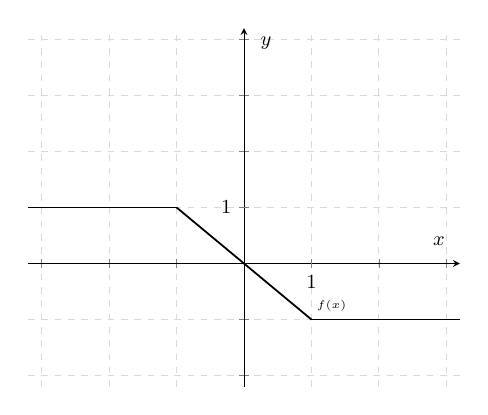
\begin{tikzpicture}[scale=0.8]
  \begin{axis}[
    axis lines=middle,
    xlabel={$x$}, ylabel={$y$},
    every axis x label/.style={at={(ticklabel* cs:0.92)}, anchor=west, yshift=10pt},
    every axis y label/.style={at={(ticklabel* cs:0.92)}, anchor=south, xshift=10pt},
    xmin=-3.2, xmax=3.2,
    ymin=-2.2, ymax=4.2,
    % 1. On définit les positions de la grille pour tous les entiers
    xtick={-3,-2,...,3},
    ytick={-2,-1,...,4},
    % 2. On masque tous les labels par défaut
    xticklabels={},
    yticklabels={},
    % 3. On ajoute spécifiquement le label "1"
    extra x ticks={1},
    extra x tick labels={1},
    extra y ticks={1},
    extra y tick labels={1},
    % Style de la grille
    grid=both,
    grid style={dashed,gray!30},
    tick label style={font=\small},
    xlabel style={font=\small},
    ylabel style={font=\small},
    % On s'assure que les extra ticks ne rajoutent pas de lignes de grille en gras
    extra tick style={grid=none}
  ]
    % f(x) = -1/7x + 11/7
  \addplot[domain=-4:-1, samples=100, thick, black]{1};
    \addplot[domain=-1:1, samples=100, thick, black]{-x};
    \addplot[domain=1:4, samples=100, thick, black]{-1}
      node[above, pos=0.1, font=\tiny] {$f(x)$};
  \end{axis}
\end{tikzpicture}
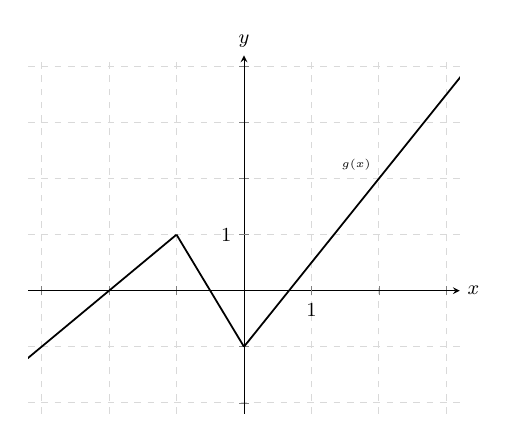
\begin{tikzpicture}[scale=0.8]
  \begin{axis}[
    axis lines=middle,
    xlabel={$x$}, ylabel={$y$},
    every axis x label/.style={at={(ticklabel* cs:1)}, anchor=west},
    every axis y label/.style={at={(ticklabel* cs:1)}, anchor=south},
    xmin=-3.2, xmax=3.2,
    ymin=-2.2, ymax=4.2,
    % 1. On définit les positions de la grille pour tous les entiers
    xtick={-3,-2,...,3},
    ytick={-2,-1,...,4},
    % 2. On masque tous les labels par défaut
    xticklabels={},
    yticklabels={},
    % 3. On ajoute spécifiquement le label "1"
    extra x ticks={1},
    extra x tick labels={1},
    extra y ticks={1},
    extra y tick labels={1},
    % Style de la grille
    grid=both,
    grid style={dashed,gray!30},
    tick label style={font=\small},
    xlabel style={font=\small},
    ylabel style={font=\small},
    % On s'assure que les extra ticks ne rajoutent pas de lignes de grille en gras
    extra tick style={grid=none}
  ]
    % f(x) = -1/7x + 11/7
  \addplot[domain=-4:-1, samples=100, thick, black]{x+2};
    \addplot[domain=-1:0, samples=100, thick, black]{-2*x-1};
    \addplot[domain=0:4, samples=100, thick, black]{3/2*x-1}
      node[above left, pos=0.5, font=\tiny] {$g(x)$};
  \end{axis}
\end{tikzpicture}
\end{center}

}
\correction{
	\tcblower

}
